\chapter{Testing}
To test the performance of the trained networks a different path for the target is chosen. The shape of the new path, shown in \autoref{fig:testPath}, has a similar curvature to the training path but a different progression. This way the snake should still be able to finish the test but also faces new situations. 

\section{Test results}
First the basic setup was tested and finished the task two times without any error. In the second run the path was mirrored on the $y$-Axe. As seen in \autoref{fig:B1_A} mean angle to the ball never surpasses an absolute value of $4$ degrees which is quite impressive.
\newline
\begin{figure}[htpb]
  \centering
  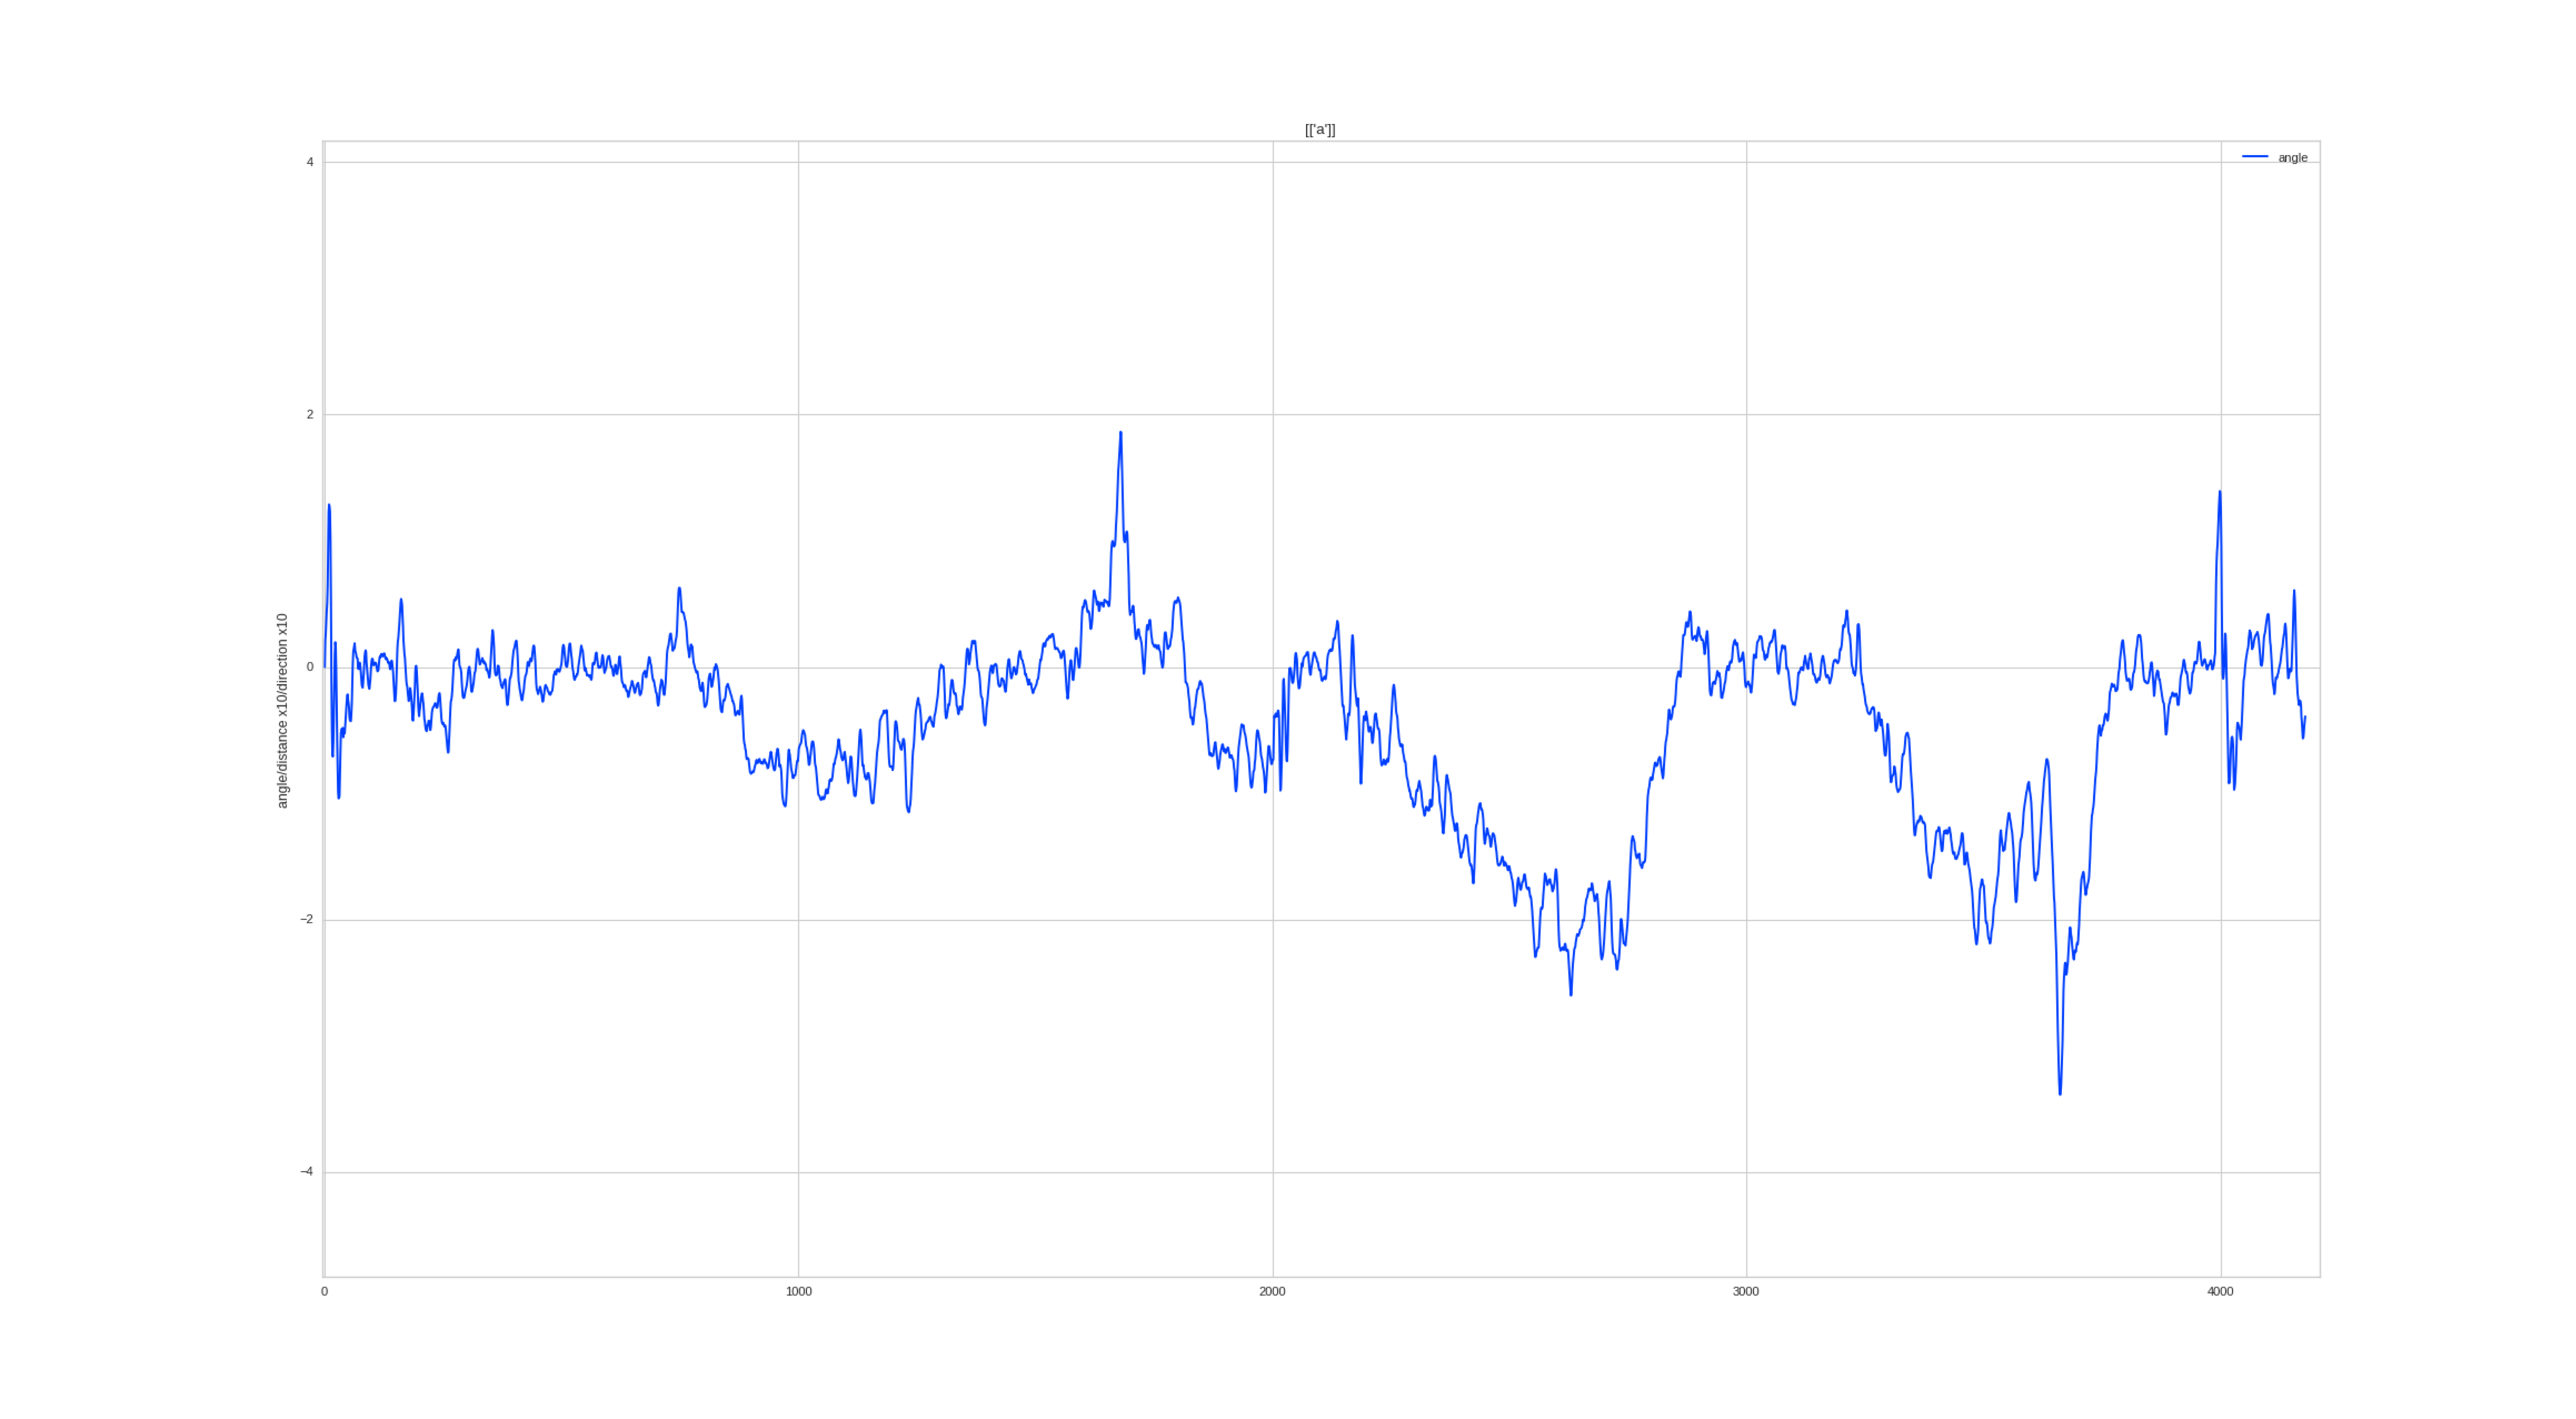
\includegraphics[width=\textwidth]{figures/plots/B1_A}
  \caption{ Performance of the basic network in the test }
  \label{fig:B1_A}
\end{figure}
Next the network with the single hidden layer was tested and even though it seemed as the weights head stabilised at the end of the training simulation, the network was not able to perform at all and never made it to the first turn. \autoref{fig:M1_perf} shows how the network fails as it has a too high affinity to go left.
\begin{figure}[htpb]
  \centering
  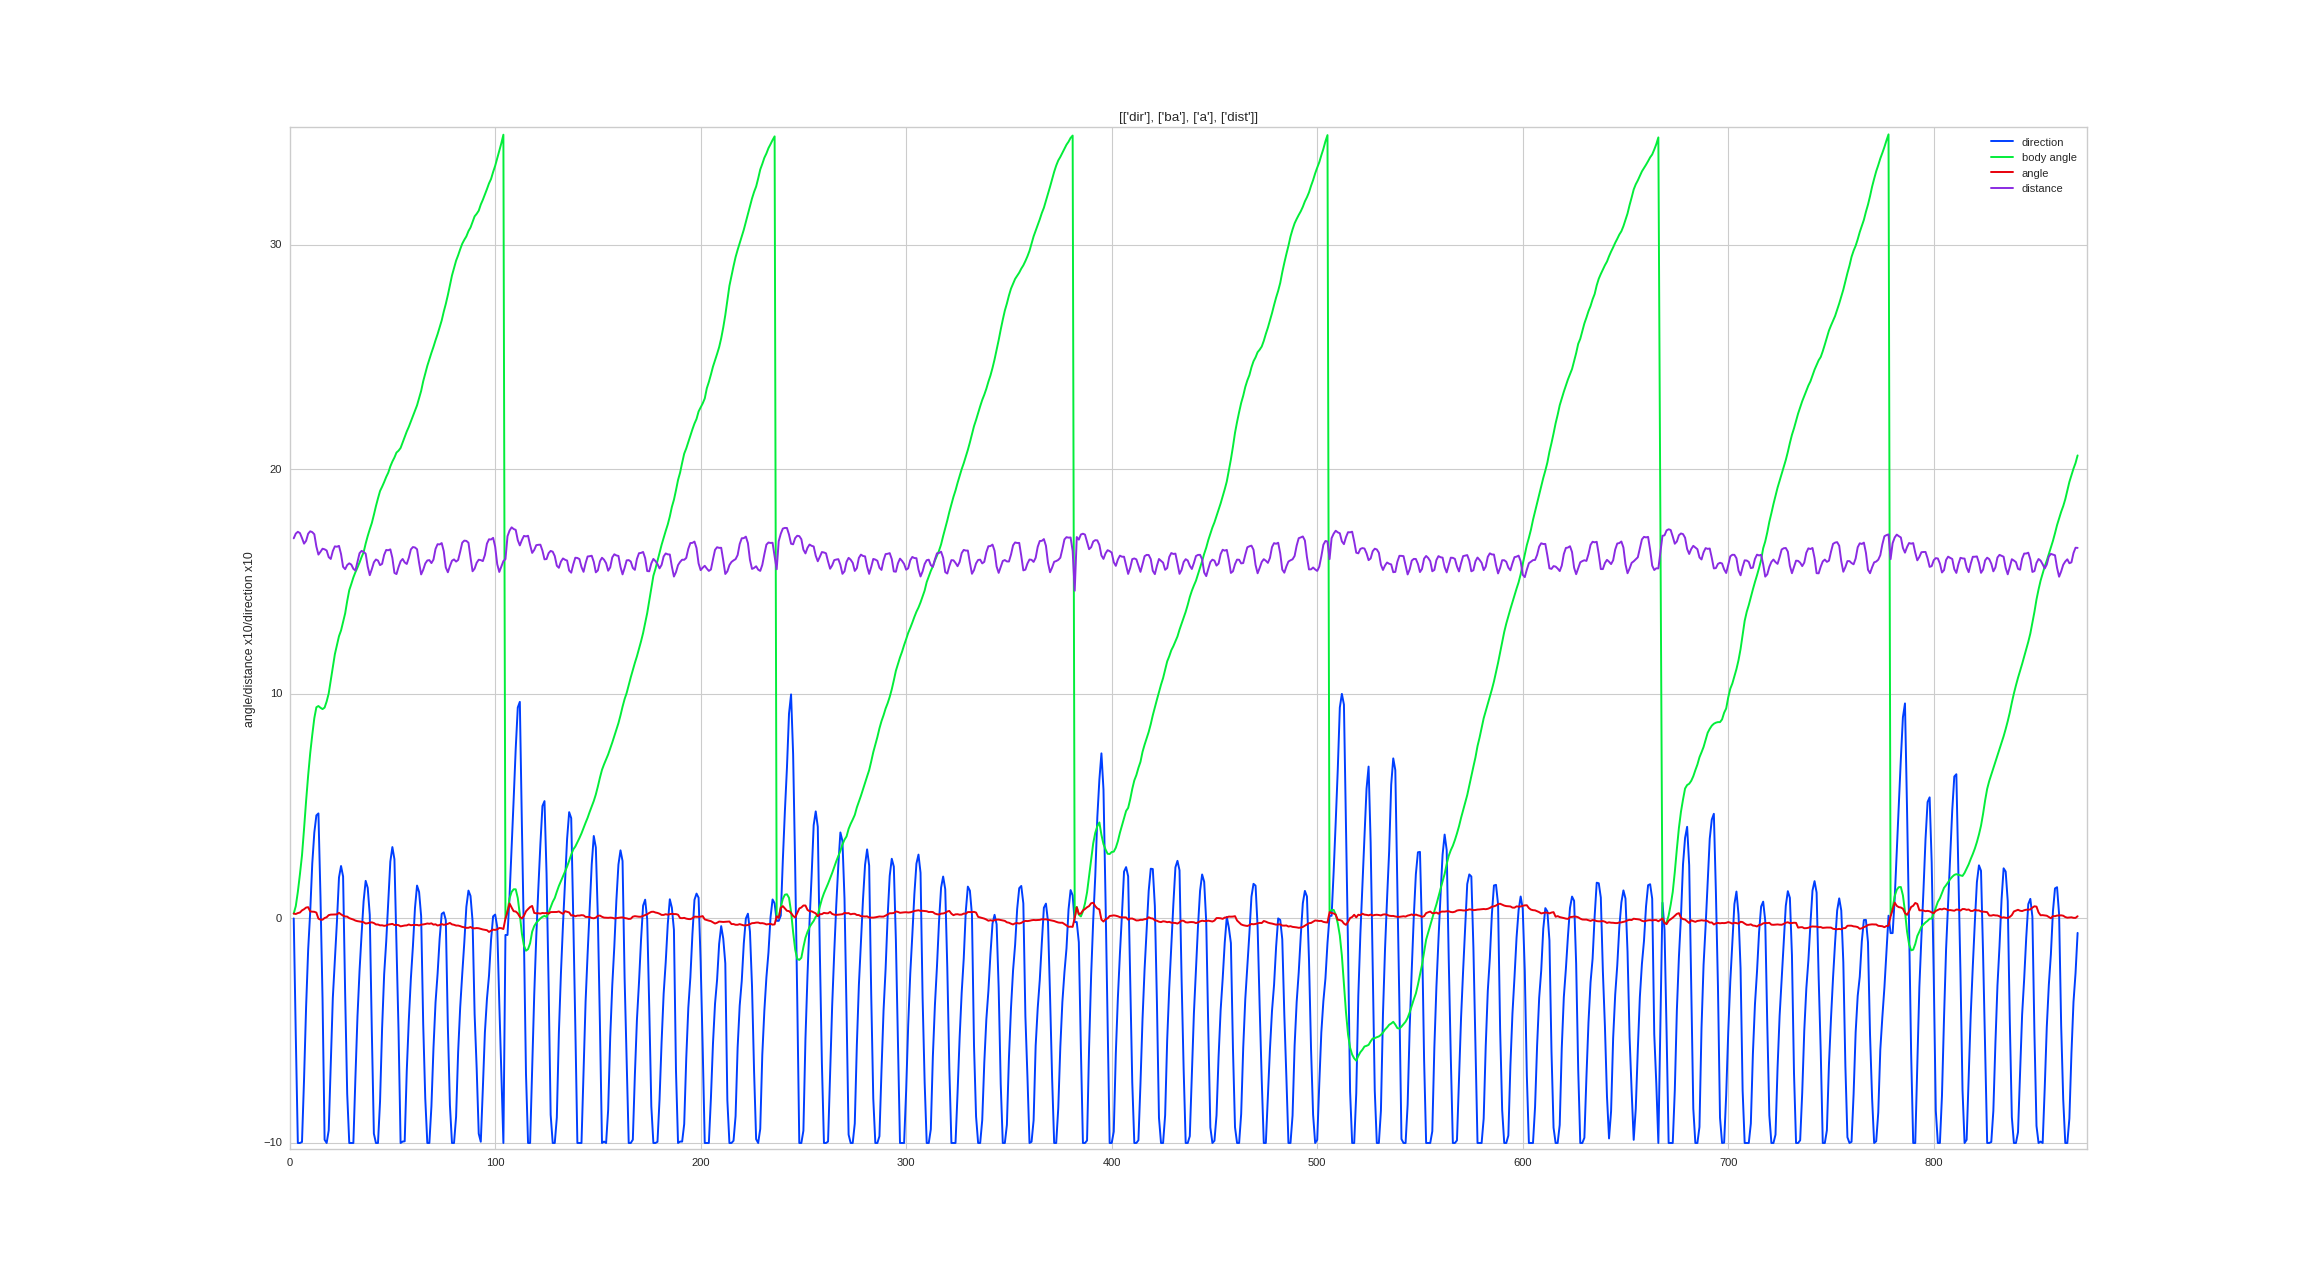
\includegraphics[width=\textwidth]{figures/plots/M1_perf}
  \caption{ Performance of the multilayer network with one hidden layer in the test }
  \label{fig:M1_perf}
\end{figure}
\newline
At last the network with the split hidden layer is tested. It performs well and keeps the mean body angl most time below $5$ degrees while its head angle is moste time lower than $1$ degree, see \autoref{fig:M2-baADist}.
\begin{figure}[htpb]
  \centering
  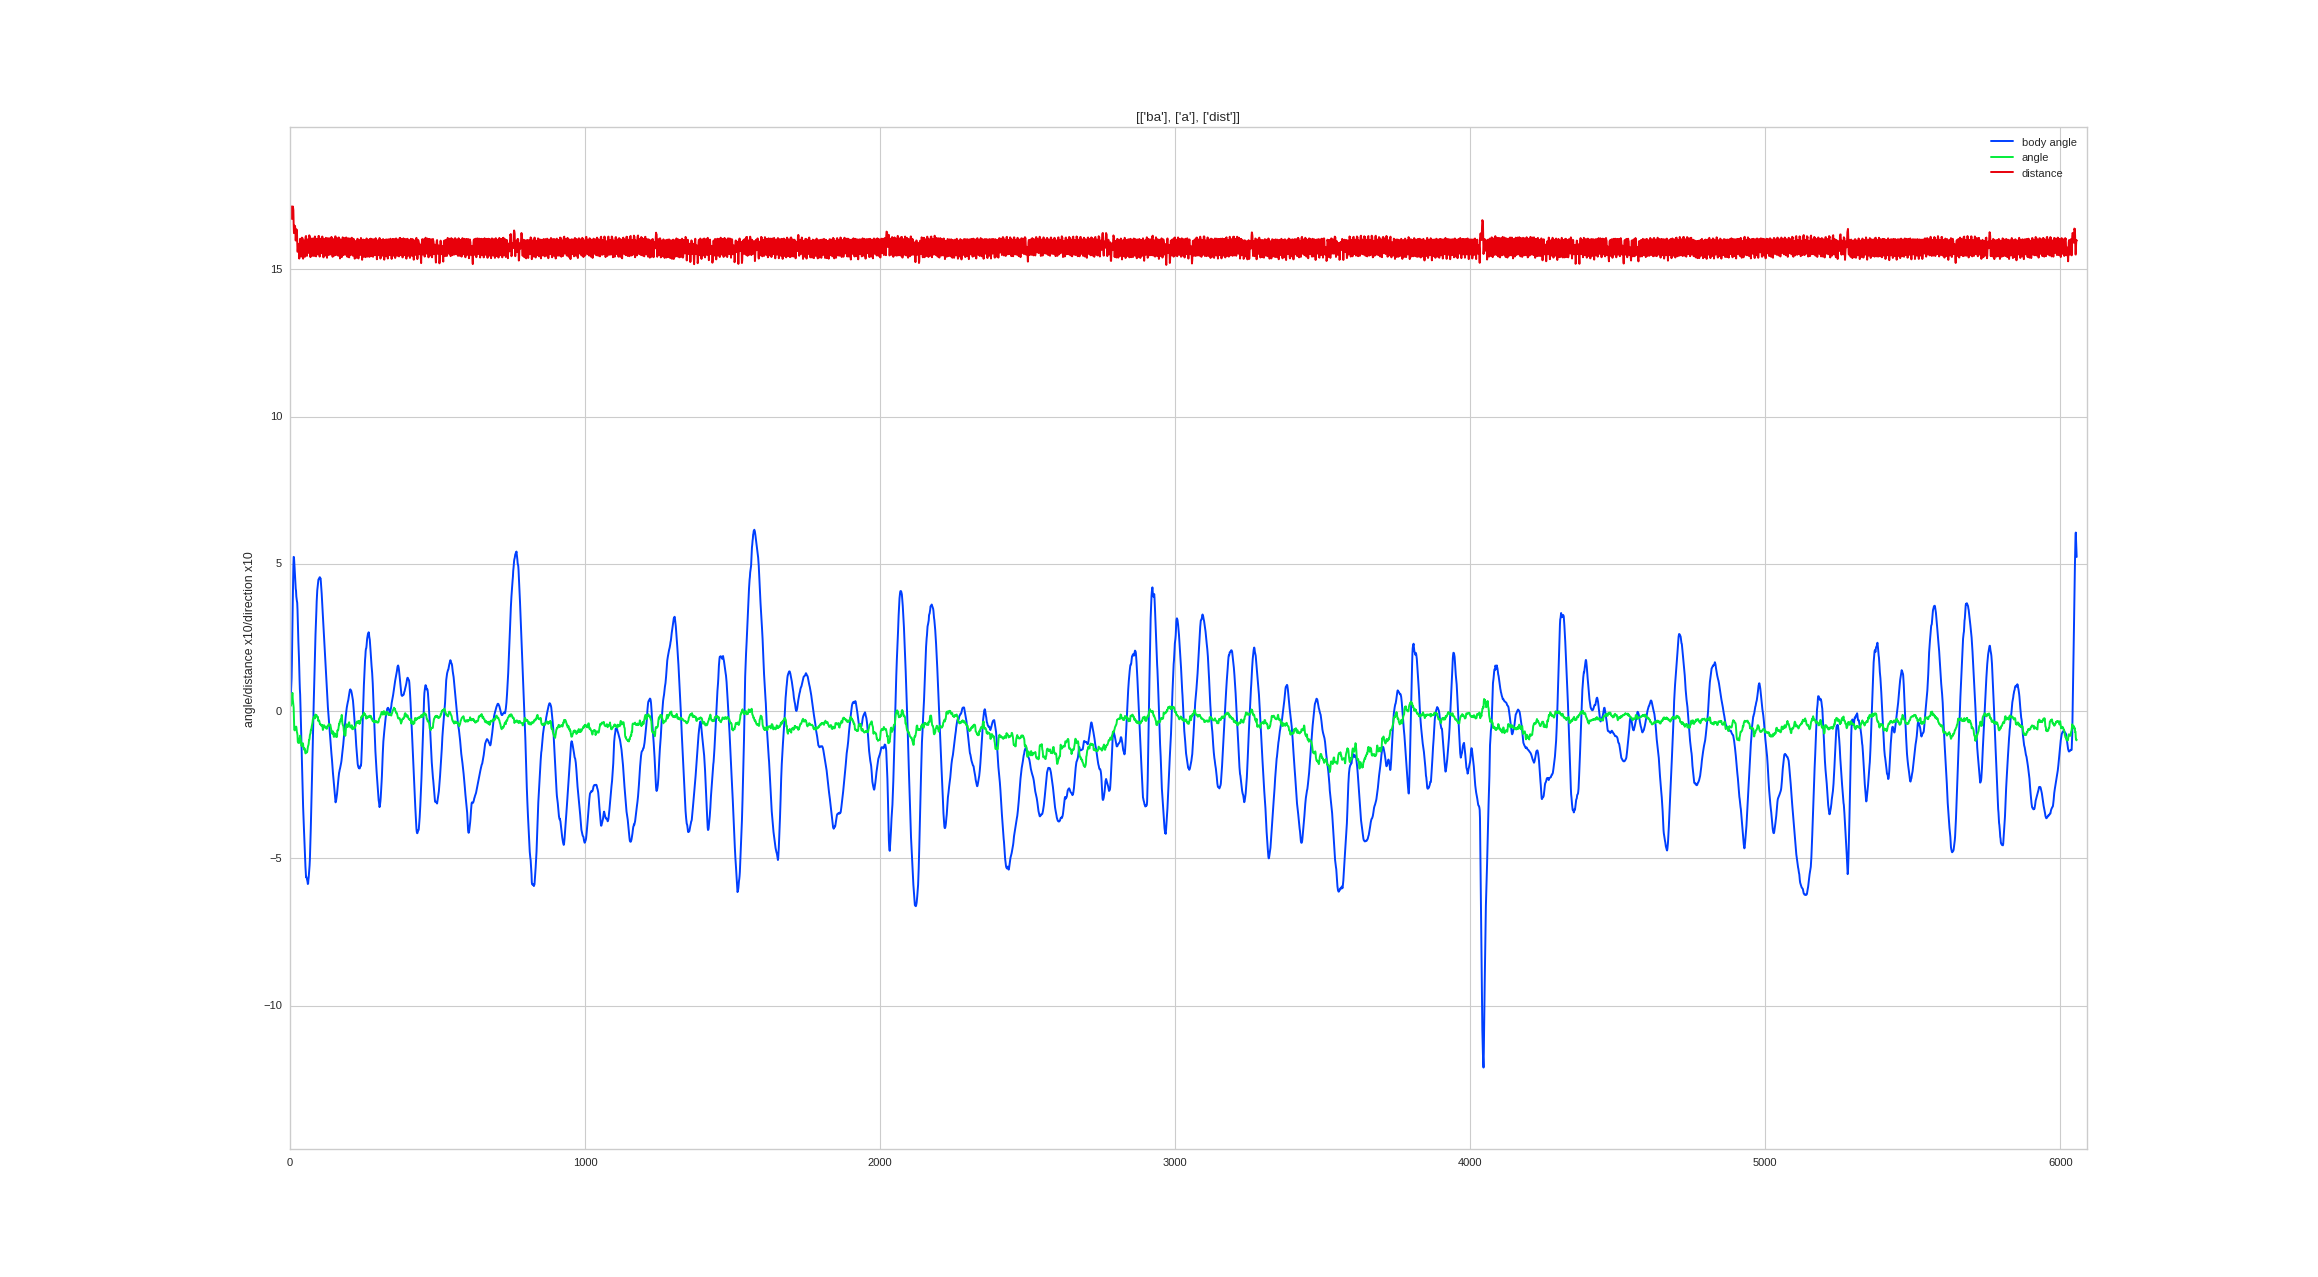
\includegraphics[width=\textwidth]{figures/plots/M2-baADist}
  \caption{ Performance of the multilayer network with the split hidden layer in the test }
  \label{fig:M2-baADist}
\end{figure}



% \begin{table}[htpb]
%   \caption[Parameters 2.Setup]{Parameters of body Neurons in the 2. setup} \label{tab:ParamsBase2N}
%   \begin{tabular}{|c| c |l|}
%       \toprule
%       Parameter & Value & Description \\
%       \midrule
%       $c_m$   & 20.0  & Capacity of the membrane \\
%       $tau_{m}$    & 50.0  & Membrane time constant \\
%       $tau_{refrac}$   & 1.  & Duration of refractory period\\
%       $v_{thresh}$   & -50.0  & Spike initiation threshold \\
%       $v_{reset}$    & -65.0  &  Reset value for $V_m$ after a spike \\
%       $v_{rest}$ & -65.0 & Resting voltage for $V_m$ \\
%       \bottomrule
%     \end{tabular}
%     \end{table}
%   \begin{table}[htpb]
%     \caption[Parameters 2.Setup]{Parameters of the body Synapses for the 2. setup} \label{tab:ParamsBase2S}
%     \begin{tabular}{|c| c |l|}
%         \toprule
%         Parameter  & Value & Description \\
%         \midrule
%         $W_{max}$ & 6000   & Maximum weight of synapse\\   
%         $W_{min}$ & -6000  & Minimum weight of synapse\\   
%         $A_{+}$   & 0.1    & Constant scaling strength of potentiation\\   
%         $A_{-}$   & -0.1   & Constant scaling strength of depression \\   
%         $\tau_c$  & 100.0   & Time constant of eligibility trace \\  
%         $\tau_n$  & 20.0   & Time constant of reward signal  \\   
%         $b$       & 0.0    & Baseline neuromodulator concentration \\    
%         \bottomrule
%     \end{tabular}
%     \end{table}


% \begin{figure}[htpb]
%   \centering
%   % This should probably go into a file in figures/
%   \begin{tikzpicture}[node distance=0.5cm]
%     \node (P0) {};
%     \node (P1) [right of=P0] {};
%     \node (P2) [right of=P1] {};
%     \node (P3) [right of=P2] {};
%     \node (P4) [right of=P3] {};
%     \node (P5) [right of=P4] {};
%     \node (P6) [right of=P5] {};
%     \node (P7) [right of=P6] {};
%     \node (P8) [right of=P7] {};
%     \node (P9) [right of=P8] {};

%     \node (I0) [below of=P0] {};
%     \node (I1) [right of=I0] {};
%     \node (I2) [right of=I1] {};
%     \node (I3) [right of=I2] {};
%     \node (I4) [right of=I3] {};
%     \node (I5) [right of=I4] {};
%     \node (I6) [right of=I5] {};
%     \node (I7) [right of=I6] {};
%     \node (I8) [right of=I7] {};
%     \node (I9) [right of=I8] {};

%     \node (O0) [below of=I0] {};
%     \node (O1) [right of=O0] {};

%     \node (D0) [below of=O0] {};
%     \node (D1) [below of=O1] {};

%     \path[every node]
%       (P0) edge (I0)
%       (P1) edge (I1)
%       (P2) edge (I2)
%       (P3) edge (I3)
%       (P4) edge (I4)
%       (P5) edge (I5)
%       (P6) edge (I6)
%       (P7) edge (I7)
%       (P8) edge (I8)
%       (P9) edge (I9)

%       (I0) edge (O0)
%       (I1) edge (O0)
%       (I2) edge (O0)
%       (I3) edge (O0)
%       (I4) edge (O0)
%       (I5) edge (O0)
%       (I6) edge (O0)
%       (I7) edge (O0)
%       (I8) edge (O0)
%       (I9) edge (O0)
      
%       (I0) edge (O1)
%       (I1) edge (O1)
%       (I2) edge (O1)
%       (I3) edge (O1)
%       (I4) edge (O1)
%       (I5) edge (O1)
%       (I6) edge (O1)
%       (I7) edge (O1)
%       (I8) edge (O1)
%       (I9) edge (O1)

%       (O0) edge (D0)
%       (O1) edge (D1);
%   \end{tikzpicture}
%   \caption[Simple Network]{Simple Network Topology}\label{fig:simpleNetwork}
% \end{figure}
